\documentclass[final]{article}

% APS360.sty enables final mode through the document-class option but does not
% define a track footer unless a NeurIPS track is selected. Course reports have
% no NeurIPS track, so provide the intentionally blank value before loading it.
\makeatletter
\providecommand{\@trackname}{}
\makeatother
\usepackage{APS360}
\setcitestyle{numbers,square}
\usepackage[utf8]{inputenc}
\usepackage[T1]{fontenc}
\usepackage{hyperref}
\usepackage{url}
\usepackage{booktabs}
\usepackage{amsmath}
\usepackage{graphicx}
\usepackage{microtype}
\usepackage{xcolor}

\title{Progress Report: Cross-Regime Generalization in Cryptocurrency Direction Prediction}
\author{%
  Bernie Fang \\
  1008726648, bernie.fang@mail.utoronto.ca \\
  \href{https://colab.research.google.com/github/Saberartoria77/APS-360-Project/blob/main/notebooks/progress_report.ipynb}{Google Colab notebook} \\
  \href{https://github.com/Saberartoria77/APS-360-Project}{GitHub repository}
}

\newcommand{\ModelParameterCount}{18067}
\newcommand{\smallhead}[1]{\vspace{0.25em}\noindent\textbf{#1}}

\begin{document}
\maketitle
\vspace{-3.5em}

\section{Brief Project Description}
Cryptocurrency forecasting is difficult because the market is continuous, volatile, nonlinear, and
non-stationary. This project studies not only whether recent market history predicts the next hourly
direction of BTC and ETH, but whether any learned signal remains reliable when the market regime
changes. Each input is a $96\times13$ tensor: 96 hourly observations described by returns, price
ranges, volume changes, RSI, MACD, Bollinger features, and rolling volatility. The output is one of
three classes---\emph{down}, \emph{flat}, or \emph{up}---defined from the next-hour close return.

Deep learning is reasonable because useful evidence may occur as short local motifs and as
longer temporal dependencies. The 1D convolution searches each window for local patterns, while an
LSTM summarizes their order and longer context. Prior work has found value in LSTMs for financial
direction prediction, while also reporting deterioration across sub-periods
\citep{fischer2018deep}; hybrid CNN--LSTM models have likewise been applied to Bitcoin
\citep{guo2021mrclstm}. This flexibility makes the model a useful subject for the eventual
cross-regime stress test, even if its first checkpoint result is modest.

\begin{center}
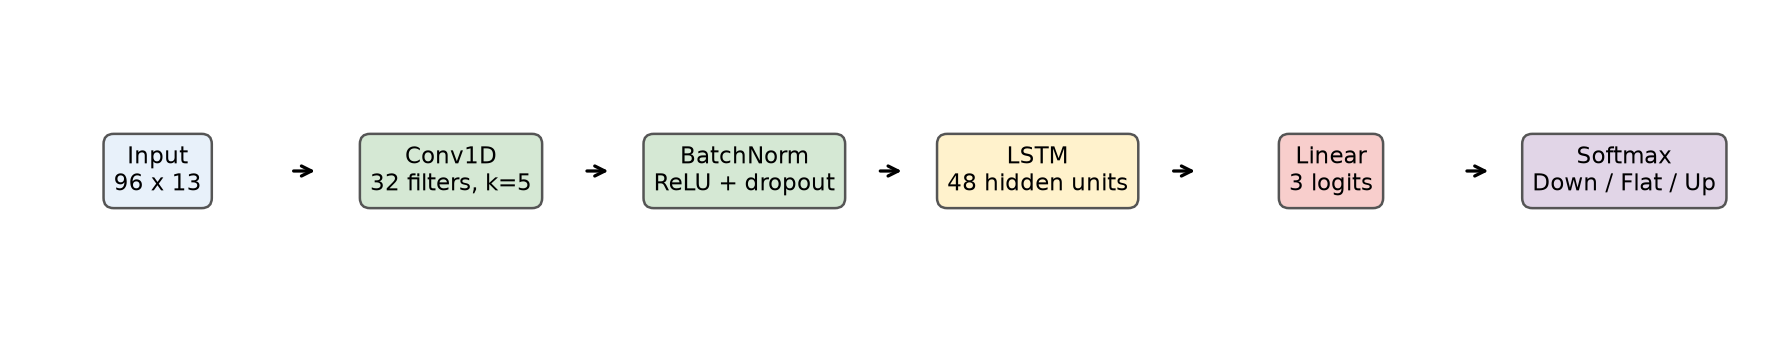
\includegraphics[width=0.98\linewidth]{artifacts/figures/model_diagram.png}
\end{center}
\vspace{-0.7em}

\section{Notable Contribution}
\subsection{Data Processing}
We downloaded 26,304 hourly Binance klines for each of BTCUSDT and ETHUSDT from July 1, 2023 to
June 30, 2026 (52,608 rows total). Rows were parsed to UTC, sorted, deduplicated, and validated for
numeric OHLCV values. We computed 13 causal features: one-hour simple/log returns, high--low range,
close--open return, volume change, RSI(14), MACD(12,26,9), Bollinger position/width(20), 24-hour
volatility, and 24-hour volume z-score. After rolling warm-up, 26,280 clean feature rows remained per
asset. A training-only median absolute next-hour return threshold (0.2357\%) defined down/flat/up.

Splits are chronological (70/15/15), windows never cross assets or split boundaries, and z-score
parameters are fitted only on usable training rows. This produced 36,584 training, 7,698 validation,
and 7,702 test windows. The main challenges were paginated API collection, class imbalance, and
preventing look-ahead leakage at feature, label, scaling, and window boundaries. Figure~\ref{fig:data}
shows the cleaned series and class statistics. For the final report, hourly observations collected
\textbf{after July 1, 2026} will be locked as never-before-seen data and \textbf{not used for tuning}.

\begin{figure}[!h]
  \centering
  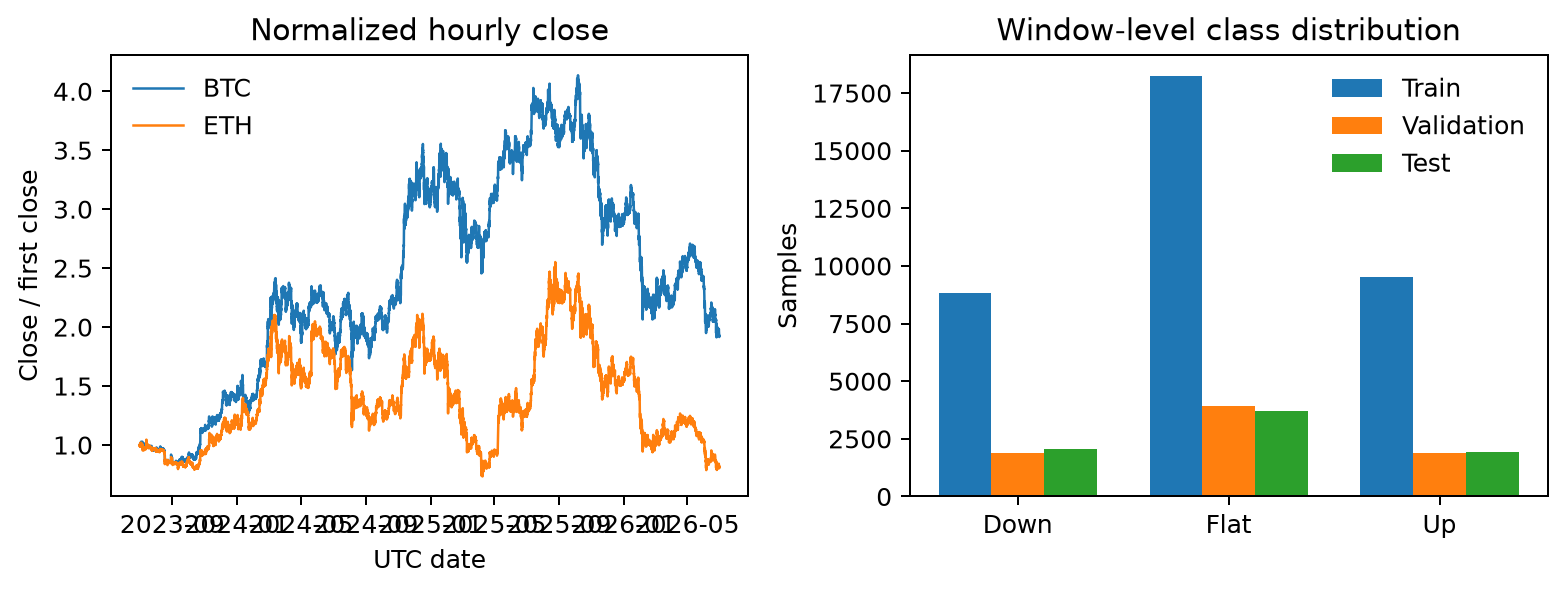
\includegraphics[width=0.92\linewidth]{artifacts/figures/data_summary.png}
  \caption{Clean hourly price paths and window-level class counts. The test set contains 2,061 down,
  3,703 flat, and 1,938 up examples.}
  \label{fig:data}
\end{figure}

\newpage
\subsection{Baseline Model}
Two deliberately simple, memory-free baselines measure whether sequence modeling adds value. The
momentum heuristic maps the most recent observed return through the same training-derived class
threshold. Logistic regression uses the final 13-feature vector, balanced class weights, and otherwise
default regularization. Both models are fitted without test-set tuning and evaluated on exactly the
same 7,702 chronological test windows as the CNN--LSTM.

\begin{table}[!h]
\centering
\small
\caption{Held-out next-hour classification results. Recall order is down/flat/up.}
\label{tab:results}
\begin{tabular}{lccccc}
\toprule
Model & Accuracy & Macro-F1 & Recall D & Recall F & Recall U \\
\midrule
Momentum & 0.421 & 0.380 & 0.295 & 0.564 & 0.281 \\
Logistic regression & \textbf{0.480} & \textbf{0.429} & 0.271 & \textbf{0.656} & 0.366 \\
CNN--LSTM & 0.444 & 0.425 & \textbf{0.403} & 0.498 & \textbf{0.386} \\
\bottomrule
\end{tabular}
\end{table}

\begin{figure}[!h]
\centering
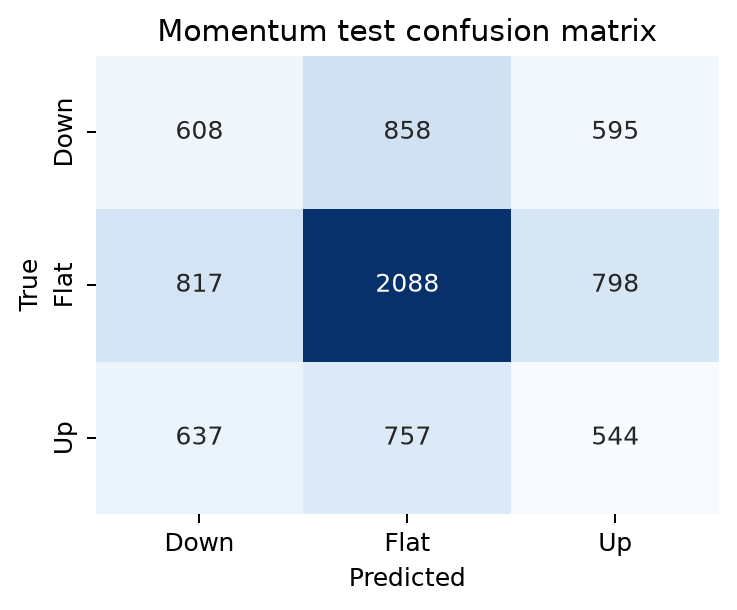
\includegraphics[width=0.32\linewidth]{artifacts/figures/confusion_momentum.png}\hfill
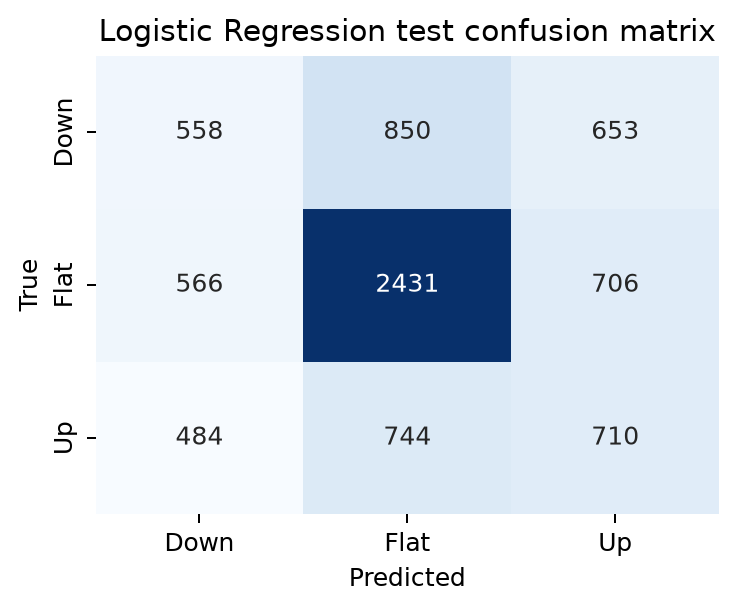
\includegraphics[width=0.32\linewidth]{artifacts/figures/confusion_logistic_regression.png}\hfill
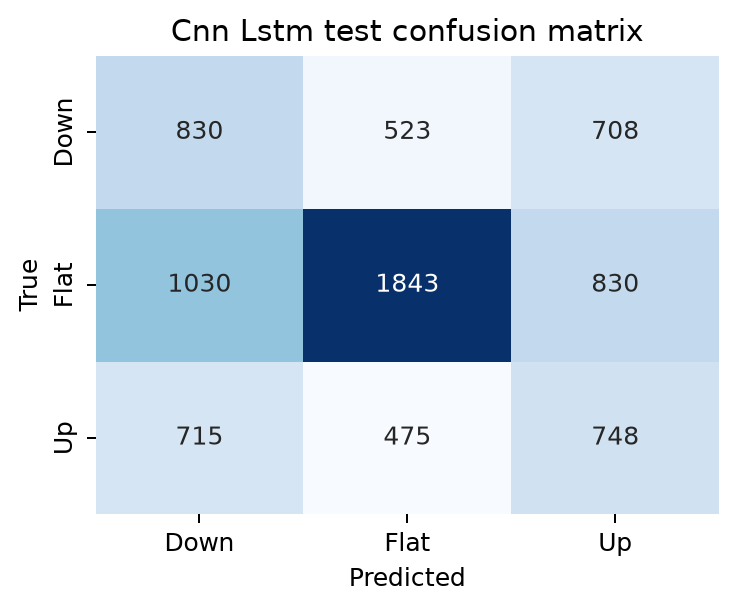
\includegraphics[width=0.32\linewidth]{artifacts/figures/confusion_cnn_lstm.png}
\caption{Test confusion matrices for momentum, logistic regression, and CNN--LSTM (left to right).}
\label{fig:confusions}
\end{figure}

\smallhead{Quantitative and qualitative result.}
Logistic regression is the strongest checkpoint by accuracy (48.0\%), improving by 5.9 percentage
points over momentum. Figure~\ref{fig:confusions} reveals why: it recognizes 65.6\% of flat examples
but only 27.1\% of down examples. Thus the apparently stronger aggregate score is concentrated in the
largest class rather than uniformly reliable directional prediction. This is a useful baseline for the
primary model because it is cheap, reproducible, and exposes whether temporal processing improves
minority-direction recall.

\smallhead{Challenge.}
The classes remain imbalanced even with a training-only, data-dependent threshold. Accuracy alone can
therefore reward predicting flat; macro-F1 and per-class recall are retained as primary companion
metrics. No metric here is interpreted as profitability.

\newpage
\subsection{Primary Model}
The PyTorch model preserves the proposal's hybrid design. A same-padded Conv1D maps 13 features to 32
channels with kernel size 5, followed by ReLU, batch normalization, and 0.15 dropout. A single LSTM
with 48 hidden units processes the 96 enriched timesteps; the final hidden output passes through 0.20
dropout and a $48\rightarrow3$ linear head. The model has \ModelParameterCount{} trainable parameters.
We use weighted cross-entropy, Adam ($10^{-3}$), batch size 256, gradient clipping at 1.0, and a fixed
seed. The maximum is 12 epochs; validation-loss patience of three selected epoch 4 and stopped after
epoch 7.

\begin{figure}[!h]
  \centering
  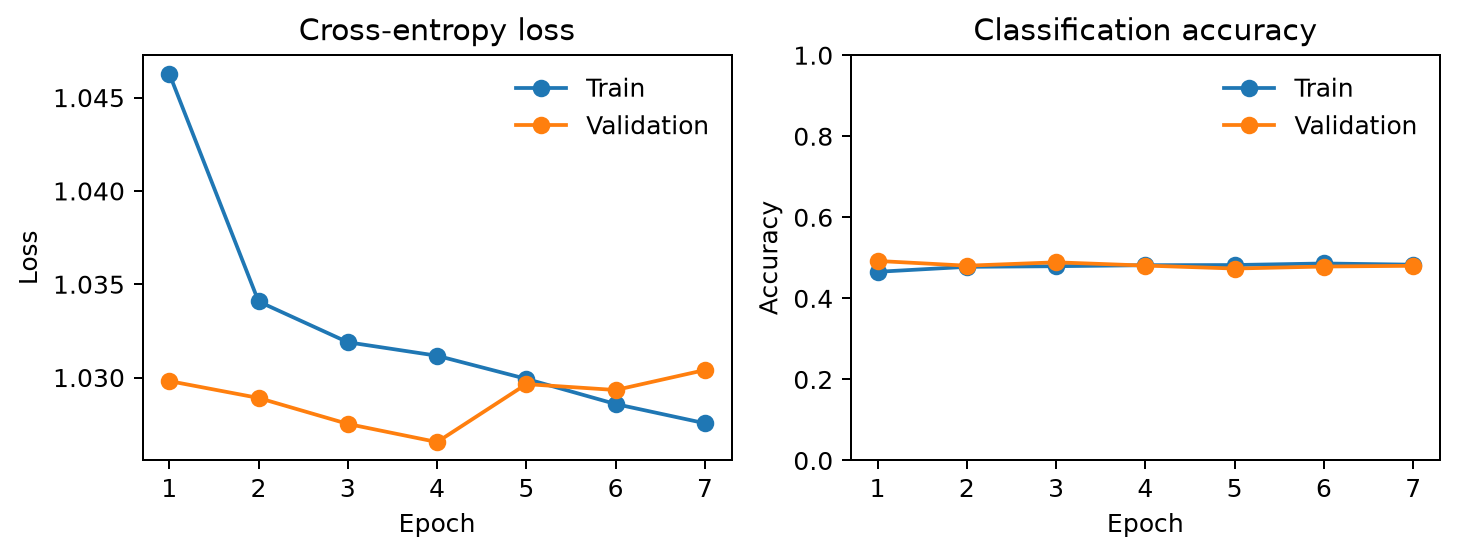
\includegraphics[width=0.82\linewidth]{artifacts/figures/learning_curves.png}
  \caption{Training and validation curves. Validation loss improved from 1.030 to 1.027 by epoch 4,
  establishing that the full neural pipeline trains, before mild divergence triggered early stopping.}
  \label{fig:learning}
\end{figure}

\smallhead{Quantitative result.}
The CNN--LSTM reaches 0.444 accuracy and 0.425 macro-F1. It \textbf{did not outperform} logistic
regression on accuracy, but improves down recall from 0.271 to 0.403 and up recall from 0.366 to 0.386.
This suggests that temporal context trades some majority-class performance for more balanced
directional sensitivity; further experiments must determine whether that trade-off survives regime
shift.

\smallhead{Qualitative result and challenge.}
The model correctly labels a BTC flat case on April 4, 2026 with 86.6\% confidence, but also labels an
actual up case on May 2 as flat with 85.9\% confidence. The most confident correct and error examples
are dominated by flat predictions, consistent with the 48.1\% flat share of the test set. Weighted loss
helps minority recall but does not remove overconfidence or non-stationarity.

\smallhead{Feasibility and next steps.}
The checkpoint demonstrates a reproducible end-to-end pipeline, two useful baselines, successful
neural optimization, and held-out quantitative/qualitative evaluation. For the final project we will
freeze the new post-July data, define volatility regimes, test cross-regime degradation, and tune only
on validation data. The current result is a feasibility study, \textbf{not trading advice}, and no
profitability claim is made.

\clearpage
\bibliographystyle{plainnat}
\bibliography{refs}

\end{document}
